% ! TeX root = ../../thesis.tex
\chapter{Implementazione}
\label{chapter:implementation}
In questo capitolo vengono affrontati gli aspetti implementativi del sistema, descrivendo le tecnologie e i paradigmi utilizzati.

\vspace*{0.5cm}

La tecnica impiegata nel sistema appartiene alla famiglia di tecniche \textit{structure-based} e si compone macroscopicamente di tre fasi, schematizzate in \Cref{img:03-system-overview}:
\begin{enumerate}
	\item \textbf{Analisi}: i sorgenti sono \textit{parsati}, preprocessati e \textit{tokenizzati};
	\item Una fase opzionale di \textbf{filtraggio};
	\item \textbf{Rilevamento} delle somiglianze.
\end{enumerate}

\begin{figure}[h!]
    \centering
    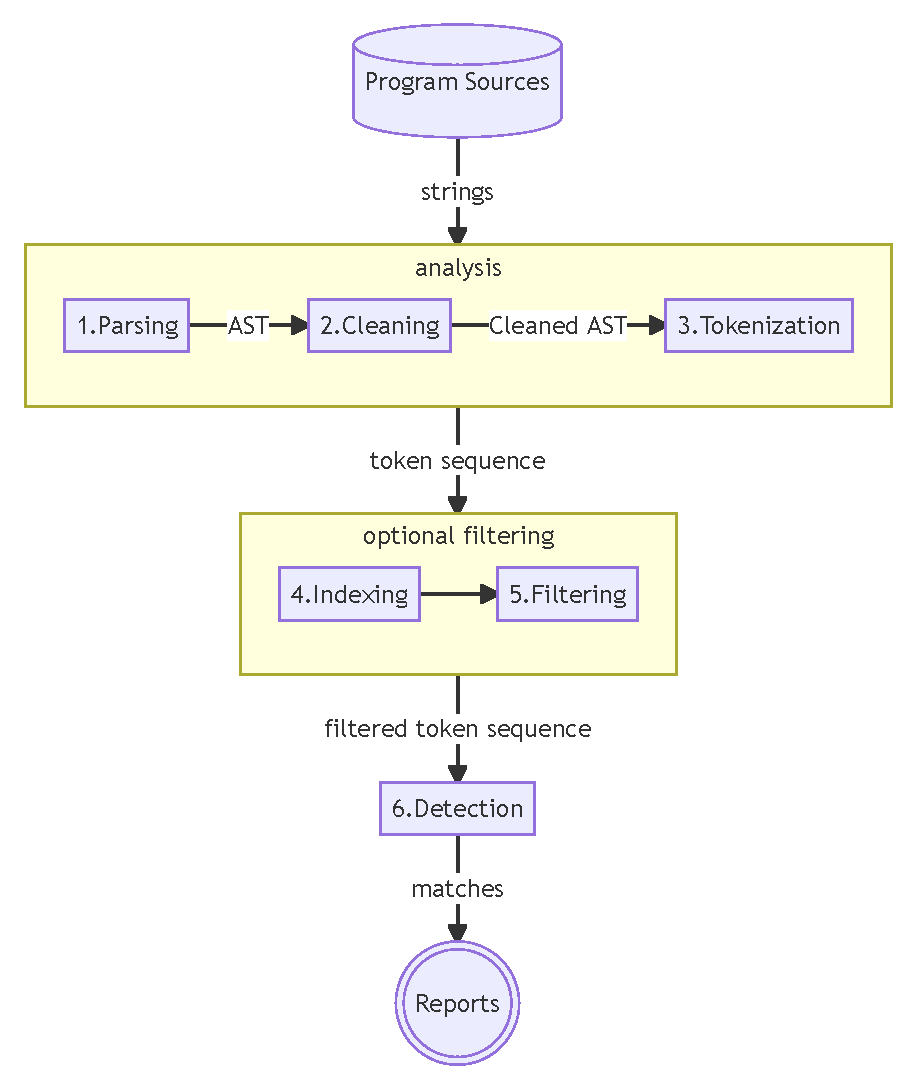
\includegraphics[width=0.8\textwidth]{resources/img/03-system-overview.pdf}
    \caption{Visione d'insieme delle fasi della tecnica impiegata nel sistema in uso.}
    \label{img:03-system-overview}
\end{figure}

Di seguito ciascuna delle tre viene approfondita.

\section{Tecnica di analisi}
Il primo passo consiste nell'effettuare il \textit{parsing} dei sorgenti, affidato alla libreria JavaParser\footnote{\url{https://javaparser.org/}}.
%
JavaParser è una libreria \textit{open source} che permette di effettuare il \textit{parsing} di codice sorgente scritto in linguaggio Java, fornendo comodi meccanismi per l'analisi e la manipolazione dello stesso.

Il risultato del \textit{parsing} è un albero sintattico equivalente a quello mostrato in \Cref{img:01-ast} che rappresenta la struttura dei sorgenti.

Tuttavia, nonostante la generazione dell'albero sintattico sollevi dalla responsabilità di eliminare dal sorgente \textit{token} superflui, come gli spazi e i punti e virgola, in quanto naturalmente modellati dalla struttura stessa dell'albero, tale AST contiene ancora informazioni sovrabbondanti, come le dichiarazioni di \texttt{import} e dei \texttt{package}.
%
Per questo motivo è necessario una fase intermedia di \textit{preprocessing} in cui l'albero viene “sfoltito”. In particolare, in questa fase l'albero viene visitato e, oltre a rimuove le dichiarazioni suddette, sono rimosse anche le funzioni \texttt{hashCode()}, \texttt{equals()} e \texttt{toString()}.
%
Queste, infatti, nella maggioranza dei casi, vengono automaticamente generate dall'\textit{IDE} e non sono rappresentative della logica dei sorgenti.

A seguire avviene la conversione del codice sorgente in una sequenza di \textit{token}.
%
Si noti che la fase di \textit{tokenizzazione} vera e propria descritta nella \Cref{01-tokenization} è già stata eseguita internamente dal \textit{parser} di JavaParser i cui \textit{token} sono quelli presenti nell'albero.
%
Tali \textit{token}, tuttavia, rappresentano in modo molto specifico la struttura del programma: ad ogni tipo del linguaggio è associato un tipo differente di \textit{token}.
%
Come descritto nella \Cref{01-tokenization} l'obiettivo è creare invece un insieme di \textit{token} "lasco" che raggruppi tipi di \textit{token} equivalenti a livello semantico.

A questo scopo, l'albero sintattico preprocessato viene visitato e, per ogni nodo, si emette un \textit{token}, con le relative informazioni circa la sua posizione nel sorgente, a seconda sia una dichiarazione semanticamente rilevante o meno.

In particolare, è stato costruito un file di configurazione \textit{Yaml}\footnote{Linguaggio, \textit{superset} di Json, per la serializzazione di dati che viene impiegato per la scrittura di file di configurazione: \url{https://yaml.org/}.} (\Cref{lst:token-config-file}) in cui sono elencati i tipi di dichiarazioni rilevanti, eventualmente tralasciando tipi troppo dettagliati, come \texttt{PrimitiveType} o \texttt{VarType}, ed aggregando tra loro dichiarazione semanticamente simili e che potrebbero essere facilmente cambiate per offuscare la copiatura.
%
Ad esempio, sono state aggregate sotto un unico tipo \texttt{loop-stmt} tutti i costrutti che effettuano un ciclo.
%
In questo modo un cambio sintattico di tipo non sarà sufficiente ad aggirare il sistema perché verrà generato lo stesso tipo di \textit{token}.
%
Si noti che questo approccio è molto flessibile e può essere "aggiustato" a piacimento nel caso sia necessario effettuare una \textit{tokenizzazione} con un insieme di \textit{token} più stringente.

\lstinputlisting[
 	language=yaml,
 	caption={Porzione del file di configurazione con la definizione dei tipi di \textit{token}},
 	label={lst:token-config-file},
]{resources/code/03-token-types.yml}

Il risultato dell'applicazione del processo sopra descritto al \Cref{lst:test-analysis} viene presentato nel \Cref{lst:result-tokenization}

\lstinputlisting[
 	caption={Risultato dell'analisi del \Cref{lst:test-analysis}},
 	label={lst:result-tokenization},
]{resources/code/03-AnalyzedTestAnalysis}

% vengono anche tolti i duplicati :)

\section{Filtraggio}
A seguito dell'analisi del codice sorgente e della generazione della sequenza di \textit{token} i sorgenti del \textit{corpus} possono essere filtrati, al fine di limitare il numero di progetti da dover confrontare.
%
Questo \textit{step} rappresenta uno snodo critico nella \textit{pipeline} di azioni da eseguire in quanto scambia una frazione dell'efficacia del sistema in favore dell'efficienza: una stima fuorviante della similarità di una coppia di progetti può comportare l'esclusione dalla comparazione degli stessi, con la conseguente perdita di sensibilità nel caso in cui rappresentassero dei veri casi di copiatura.
%
Per questo motivo la fase di filtraggio è \textit{opzionalmente} eseguita a discrezione dell'utente, che si presume possa valutare se necessita di un'analisi più veloce ma meno esaustiva o viceversa.

Come già presentato nella \Cref{01-tokenization}, il processo di filtraggio è preceduto da una fase d'indicizzazione in cui vengono aggregati i dati sotto forma di una struttura dati per mezzo della quale è possibile estrarre informazioni statistiche significative per la stima della similarità.

Nel sistema è attualmente implementato un indice equivalente a quello presentato in \Cref{table:token-indexing} a partire dal quale la similarità tra progetti è stata calcolata mediante la \textbf{similarità coseno}.
%
Essa è una metrica euristica ampiamente utilizzata nel contesto dell'analisi testuale che misura la similutidine di due vettori calcolando il coseno del loro angolo: 
\begin{equation}
	cosine\_similarity(A,B) = \frac{A \cdot B}{||A|| ||B||} 
		= \frac{\sum_{k=1}^{n} A(k) B(k)}{\sqrt{\sum_{k=1}^{n}A(k)^2 \cdot \sum_{k=1}^{n} B(k)^2}}
\end{equation}
dove $A$ e $B$ sono due vettori di attributi numerici a $n$ dimensioni.

In generale, il risultato della similarità è un valore compreso tra $-1$ e $1$ dove $-1$ indica che i due vettori sono \textit{anti}-correlati (hanno verso opposto), $1$ indica massima correlazione e $0$ un'assenza di correlazione (i due vettori sono ortogonali tra loro).

Nel nostro caso, il contenuto dei due vettori è la frequenza dei tipi di \textit{token} in cui il $k$-esimo elemento contiene il numero di volte in cui il $k$-esimo tipo di \textit{token} ricorre nel sorgente, oppure $0$ se non presente.
%
Poiché le frequenze sono valori sempre positivi, nel caso in esame, si otterranno valori compresi tra $0$ e $1$, dove $1$ indica che i tipi di \textit{token} contenuti nelle due rappresentazioni sono gli stessi, presenti in egual numero ma non necessariamente disposti nello stesso ordine, e $0$ indica che non c'è alcun tipo di \textit{token} comune.

A seguito della stima della similarità coseno, tutte le coppie di rappresentazioni la cui similarità è inferiore a un valore di soglia sono esclusi.
%
Tale valore è calcolato, seguendo quanto riportato in \cite{es-plag}, utilizzando la formula riportata nell'\Cref{eq:cosine-filtering-threshold}.

\begin{equation}
\label{eq:cosine-filtering-threshold}	
	threshold = sim_{min} + init\_threshold \cdot (sim_{max} - sim_{min})
\end{equation}

dove $init\_threshold$ è un valore compreso tra $0$ e $1$ (corrispondente al range $0-100\%$) e $sim_{max}$ e $sim_{min}$ sono rispettivamente la similarità coseno massima e minima risultante dalla comparazione di tutte le coppie.

Secondo le valutazioni presentate in \cite{es-plag} questo tipo di filtraggio aumenta l'efficienza del sistema con un compromesso in termini di efficacia che rimane accettabile fintanto che la soglia $init\_threshold$ è mantenuta al di sotto del 60\%.

\section{Rilevamento delle somiglianze}
\label{03-matching-algorithms}
Gli algoritmi impiegati per confrontare due sequenze di \textit{token} sono il \textit{Greedy String Tiling} e il \textit{Running Karp-Rabin Greedy String Tiling}, che ne rappresenta una sua evoluzione, introdotti da M. Wise nel 1993 in \cite{wise-running-93} a seguito della necessità di sviluppare proprio un sistema automatico antiplagio, anche se negli anni successivi gli stessi algoritmi sono stati impiegati in altri campi, tra cui il confronto di sequenze di proteine/DNA.

Sebbene questi siano stati concepiti per lavorare su sequenze di stringhe, possono essere facilmente riadattati per operare su sequenze di \textit{token}

Dette $A$ e $B$ due sequenze di \textit{token}, un algoritmo per misurare la similarità in questo dominio deve determinare una sottosequenza comune che abbia le seguenti proprietà:
\begin{itemize}
	\item ogni \textit{token} di $A$ può essere abbinato solo con esattamente un solo \textit{token} di $B$;
	\item le sottosequenze comuni devono essere trovate indipendentemente dalla loro posizione nel sorgente;
	\item le sottosequenze più lunghe sono preferite a quelle più piccole, in quanto le sottosequenze brevi è molto probabile rappresentino casi spuri.
\end{itemize}

L'algoritmo si compone principalmente di due fasi:
\begin{itemize}
	\item \textbf{Fase 1}: in questa fase, viene ricercata la corrispondenza più lunga. Questo è fatto grazie un triplo ciclo innestato: il primo itera sui token della sequenza più corta, denominata \textit{pattern}, il secondo compara ciascuno di questi con ogni \textit{token} della sequenza più lunga, denominata \textit{text}. Se i due \textit{token} corrispondono il ciclo più interno cerca di estendere il \textit{match} il più possibile (fermandosi non appena trova un \textit{token} che nelle due sequenze differisce).

	\item \textbf{Fase 2}: questa fase marca ciascun natch di lunghezza massima (\textit{maximal match}) trovato nella fase precedente. Questo garantisce che ciascun \textit{token} venga usato per un solo \textit{match} e divenga indisponibile per i \textit{match} successivi (che hanno una minor lunghezza). Nella terminologia di \cite{wise-running-93} i \textit{match} i cui \textit{token} sono stati marcati sono denominati \textit{tile}. Si noti che, anche se un \textit{match} è parzialmente occluso e perciò non viene marcato, una versione più corta dello stesso \textit{match} può essere marcato durante le successive iterazioni.
\end{itemize}

Queste due fasi vengono ripetute fino a quando non vengono trovate più corrispondenze di lunghezza almeno \texttt{minimum\_match\_length}.
%
Tale valore è imposto per non generare troppe sequenze spurie di lunghezza irrisoria e garantire risultati migliori.
%
Giacché la lunghezza dei \textit{match} diminuisce ad ogni iterazione è garantito che l'algoritmo termini.

Lo pseudocodice dell'algoritmo è presentato nel \Cref{lst:gst}.

\lstinputlisting[
	language=pseudocode,
 	caption={Pseudocodice dell'algoritmo \textit{Greedy String Tiling (GST)}. In accordo con la terminologia del \textit{paper} $P$ rappresenta il \textit{pattern} ovvero la sequenza da confrontare più corta, mentre $T$ il \textit{text} ovvero la sequenza tra le due più lunga.},
 	label={lst:gst},
]{resources/code/03-gst}

Questo algoritmo è dimostrato \cite{wise-running-93} essere ottimo in termini di massimizzazione della copertura delle stringhe.
%
Nonostante ciò, nel caso peggiore, ha una complessità $O(n^3)$ e pertanto è molto inefficiente.

Per far fronte a questo problema è stato ideato un nuovo algoritmo chiamato \textit{Running Karp Rabin Greedy String Tiling}.
%
L'idea su cui si fonda per velocizzare il confronto è impiegare una funzione di \textit{hashing}.
%
In particolare, il valore di \textit{hash} di ogni sottosequenza di lunghezza $s$ del \textit{pattern} viene confrontato con il valore di \textit{hash} di quelle del \textit{text}.
%
Laddove i due valori corrispondano, e solo in questo caso, le sottosequenze vengono confrontate \textit{token} per \textit{token} per assicurarsi che effettivamente siano uguali e non frutto di una collisione della funzione di \textit{hash}.

Nel \Cref{lst:rkr-scanpattern} viene mostrato lo pseudocodice della \textit{routine} che si occupa di effettuare questo confronto.
%
Come si può osservare, nelle righe 1-3 vengono calcolati i valori di \textit{hash} di tutte le sottosequenze (non marcate) di lunghezza $s$ del \textit{text} e vengono salvati in una \textit{hashtable}, una mappa con le corrispondenze sottosequenza di \textit{token}-valore di \textit{hash}.
%
Lo stesso viene fatto per il \textit{pattern} con la differenza che, non appena calcolato il valore \textit{hash} per la sottosequenza considerata, si verifica se lo stesso sia già presente nella \textit{hashtable}.
%
In questo caso, infatti, potrebbe effettivamente esserci una corrispondenza e si procede verificando \textit{token} per \textit{token}.
%
Si noti che nei casi in cui la corrispondenza sia effettiva e non sia causata da un artefatto della funzione di \textit{hash}, il \textit{match} è esteso fino al primo \textit{token} non corrispondente, proprio come nel precedente algoritmo.

\lstinputlisting[
 	language=pseudocode,
 	caption={Pseudocodice della \textit{routine} \texttt{scanpattern} dell'algoritmo \textit{RKR-GST}},
 	label={lst:rkr-scanpattern},
]{resources/code/03-rkr-gst-scanpattern}

Nella versione originale dell'algoritmo la struttura dati utilizzata per memorizzare i \textit{match} è una lista di code in cui ogni coda memorizza i \textit{match} della stessa lunghezza, mantenuta ordinata per valori descrenti.

Il \Cref{lst:rkr-markarrays} presenta lo pseudocodice della \textit{routine} che effettua la marcatura dei \textit{match} individuati nella \textit{routine} \texttt{scanpattern}, corrispondente alla seconda fase dell'algoritmo precedente.
%
La principale differenza con la precedente versione risiede nel fatto che la marcatura viene effettuata per ogni \textit{match} e non solo per quelli di lunghezza massima.
%
Inoltre, se il \textit{match} risulta parzialmente occluso, ma la rimanente parte non occlusa è  di lunghezza $m > s$, questa viene salvata nella lista di code, in modo tale da essere valutata nella successiva iterazione in cui vengono valutati tutti i \textit{match} di lunghezza $m$ (righe 11-13).

\lstinputlisting[
 	language=pseudocode,
 	caption={Pseudocodice \textit{routine} \texttt{markarrays} dell'algoritmo \textit{RKR-GST}},
 	label={lst:rkr-markarrays},
]{resources/code/03-rkr-gst-markarrays}

Infine, nel \Cref{lst:rkr-top-level} è mostrato l'\textit{entry-point} dell'algoritmo.
%
Come si può osservare, corrispondenze molto lunghe vengono trovate solo durante la prima iterazione: dopo di questa, infatti, non è possibile siano trovate corrispondenze maggiori del doppio della lunghezza di ricerca corrente.
%
Questo garantisce che, nelle successive iterazioni, l'algoritmo termini.

\lstinputlisting[
 	language=pseudocode,
 	caption={\textit{Entry-point} dell'algoritmo \textit{RKR-GST}},
 	label={lst:rkr-top-level},
]{resources/code/03-rkr-gst-top-algorithm}

Il valore di $s$ (l'equivalente di \texttt{minimum\_match\_length} nell'algoritmo \textit{GST}) è scelto in modo tale da garantire che non vengano cercate corrispondenze troppo piccole.
%
Un valore plausibile di $s$ consigliato in \cite{wise-running-93} è 20.

Sebbene la complessità di questo algoritmo sia dimostrato essere, nel caso peggiore, $O(n^2)$, nel caso medio la complessità è pressoché \textbf{lineare}.
%
Ciò migliora notevolmente le prestazioni rispetto all'algoritmo \textit{Greedy String Tiling}.

\section{Stima della similarità}

\subsection*{Similarità tra due sorgenti}
La misura della similarità di due sorgenti dovrebbe intuitivamente riflettere la frazione di \textit{token} dei programmi originali che sono "coperti" da \textit{match}.
%
Seguendo questo principio ci sono due possibili scelte che possono essere intraprese e che determinano la formula di stima di similarità: se si vuole che la similarità del 100\% significhi che le due sequenze sono identiche dobbiamo considerare entrambe le stringhe nel computo, come segue:
%
\begin{equation}
\label{eq:max-norm-sim}
	sim(A, B) = \frac{2 \cdot \sum_{match \in tiles} length}{|A|+|B|}
\end{equation}
%
Se, invece, preferiamo che ogni programma che è stato copiato completamente(e poi magari esteso) produca una similarità del 100\%, dobbiamo considerare solo la sottosequenza più corta:
%
\begin{equation}
\label{eq:avg-norm-sim}
	sim(A, B) = \frac{\sum_{match \in tiles} length}{min(|A|, |B|)}
\end{equation} 

Per mitigare il problema dell'insensibilità al riordino delle sottosequenze di cui è intrinsicamente affetta la tecnica di analisi impiegata, in \cite{es-plag} viene proposto di modificare la formula di stima della similarità introducendo un meccanismo di penalità ispirato dal principio che, solitamente, un numero elevato di sottosequenze comuni si verifica proprio a causa del riordino delle stesse. 
%
Applicando pertanto una penalità proporzionata al numero di sottosequenze comuni, maggiore sarà il numero di sottosequenze individuate, minore sarà il grado di similarità determinato.
%
Le formule aggiornate sono di seguito presentate.

\begin{equation}
	sim(A, B) = \frac{2 \cdot \bigl( \sum_{match \in tiles} length - (|tiles|-1) \bigr)}{|A|+|B|}
\end{equation}

\begin{equation}
	sim(A, B) = \frac{\sum_{match \in tiles} length - (|tiles|-1)}{min(|A|, |B|)}
\end{equation} 

\subsection*{Similarità tra due progetti}

\section{Strumenti di sviluppo}

\subsection*{\textit{Kotlin}}
Il progetto è stato sviluppato interamente in \textit{Kotlin}, un linguaggio di programmazione \textbf{orientato agli oggetti} e \textbf{funzionale} \textit{open source}\footnote{\url{https://github.com/JetBrains/kotlin}} progettato e gestito da \textit{JetBrains}\footnote{\url{https://www.jetbrains.com/}} a partire dal 2010.
%
Si tratta di un linguaggio multipiattaforma compilato, tipato staticamente e  completamente interoperabile con \textit{Java} e la \textit{JVM} e \textit{Android}, applicabile in una vasta gamma di ambiti, dallo sviluppo \textit{server side} a quello di applicazioni mobili (attualmente è il linguaggio di riferimento per \textit{Android}, avendo surclassato Java).
%
Inoltre, oltre a Java e Android, \textit{Kotlin} può essere compilato in \textit{JavaScript}, consentendo di eseguire codice \textit{Kotlin} nel \textit{browser}.

L'obiettivo principale del linguaggio è fornire un'alternativa a Java più concisa, produttiva e sicura, adatta in tutti i contesti in cui è tutt'oggi utilizzato.
%
Infatti, essendo completamente compatibile con Java, sfrutta tutte le sue numerose librerie, estendendole e garantendo le stesse \textit{performance}.

I tratti distintivi di \textit{Kotlin} sono certamente la sua espressività e concisione, che permettono di sviluppare codice che rivela l'intento senza oscurarlo con codice verboso per specificare come viene realizzato.

\begin{figure}[h]
    \centering
    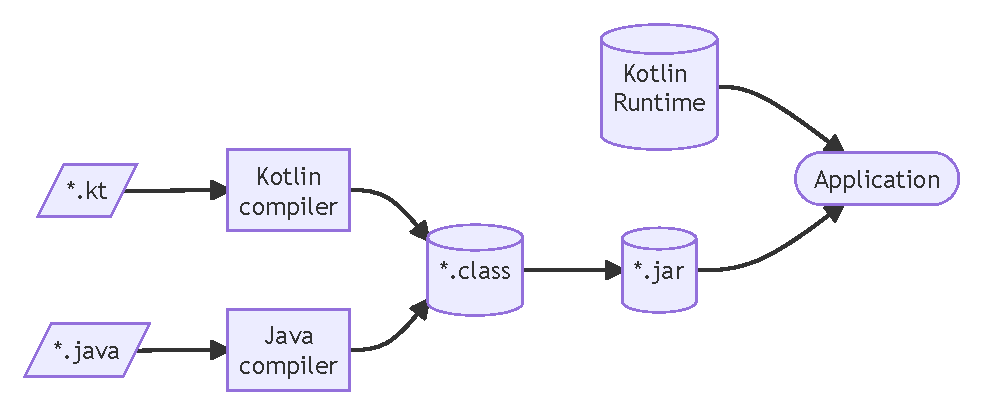
\includegraphics[width=0.8\textwidth]{resources/img/03-kotlincompilation.pdf}
    \caption{Processo di compilazione di \textit{Kotlin}.}
    \label{img:03-kotlin-compilation}
\end{figure}

\subsection*{Git e \textit{CI/CD}}
Per lo sviluppo del progetto, si è utilizzato Git, uno \textit{standard de facto} nell'ambito dei sistemi di controllo di versione decentralizzato, che permettere di tenere traccia dello storico delle modifiche e lo sviluppo simultaneo da parte di più sviluppatori, senza che questi debbano sobbarcarsi la gestione dell'intero progetto a mano, con tutti i conseguenti problemi.

In particolare, il \textit{workflow} adottato è il seguente: il progetto è mantenuto in una \textit{repository} pubblica centrale\footnote{\url{https://github.com/DanySK/code-plagiarism-detector}} e ciascun sviluppatore lavora su una \textit{working copy} (\textit{fork}).
%
Non appena una \textit{feature} è completata o si arriva a un buon grado di sviluppo si aprono delle \textit{pull request}, nelle quali i contributi sono revisionati per accertarsi passino i controlli di qualità.
%
Questi vengono eseguiti automaticamente grazie all'utilizzo delle \textit{GitHub Actions}, una piattaforma di \textit{Continuous Integration and Delivery} (CI/CD) che permette di automattizare il processo di \textit{testing}, \textit{building} e \textit{deployment}.
%
Tramite un file di configurazione \textit{Yaml} è possibile definire uno o più \textit{workflow} che effettuino i controlli desiderati utilizzando ... su più sistemi operativi.

Processo di build con aggiornamento delle dipendenze

\subsection*{Librerie esterne}
Per lo sviluppo complessivo del progetto sono state impiegate le seguenti librerie:
\begin{itemize}
	\item \textbf{JavaParser}\footnote{\url{https://javaparser.org}} per effettuare l'analisi dei sorgenti sviluppati in linguaggio Java;
	\item \textbf{Github API for Java}\footnote{\url{https://github-api.kohsuke.org}} per interagire con l'API di GitHub e recuperare le \textit{repository}. Per recuperare i progetti caricati su \textit{Bitbucket}, non essendoci di una libreria pronta all'uso, si è utilizzata \textbf{Unirest} per effettuare le richieste HTTP;
	\item \textbf{JGit}\footnote{\url{https://www.eclipse.org/jgit/}} per lo scaricaramento (\textit{clone}) dei progetti da \textit{GitHub} e \textit{Bitbucket}.
	\item \textbf{Clikt}\footnote{\url{https://ajalt.github.io/clikt/}} per la scrittura dell'interfaccia da riga di comando;
	\item \textbf{Kaml}\footnote{\url{https://github.com/charleskorn/kaml}} per la (de)serializzazione di file di configurazione \textit{Yaml}.
	\item \textbf{Kotest}\footnote{\url{https://kotest.io}} e \textbf{Mockk}\footnote{\url{https://mockk.io}} per effettuare e agevolare la scrittura di \textit{test}.
\end{itemize}

\subsection*{Controllo di qualità}
Il controllo di qualità del \textit{software} è eseguito medianti strumenti automatici, di seguito elencati, che hanno l'obiettivo di evidenziare potenziali problemi o possibili miglioramenti:
\begin{itemize}
	\item \textbf{Detekt}: 
	\item \textbf{Klint}:
	\item ...
	\item \textbf{CPD}:
\end{itemize}
